
% "Станет проще"

\documentclass[a4paper,12pt]{article} % тип документа
\usepackage{cmap}
% report, book

%  Русский язык

\usepackage[T2B]{fontenc}			% кодировка
\usepackage[utf8]{inputenc}			% кодировка исходного текста
\usepackage{graphicx}
\usepackage[english,russian]{babel}	% локализация и переносы


%отступ
\usepackage[left=3cm,right=3cm,
    top=2cm,bottom=2cm,bindingoffset=0cm]{geometry}

% Математика
\usepackage{amsmath,amsfonts,amssymb,amsthm,mathtools}
\usepackage{csvsimple}
\usepackage{multirow}
\usepackage{wasysym}
\usepackage{subcaption}
\usepackage{verbatim}
%\usepackage{ae,aecompl} better q
\usepackage{float}
\usepackage{enumerate}
\usepackage[dvipsnames]{xcolor}
\usepackage{rotating}
\usepackage[hidelinks]{hyperref} % Hide links

%Заговолок
\graphicspath{ {img/} }


\begin{titlepage}
\author{Михаил}
\title{План работ по тесту системы адресации я ячейкам.}
\date{\today}
\end{titlepage}



\begin{document} % начало документа

\maketitle
Приветствую! Далее я в крадце опишу, что можно попробовать сделать.
\section{Цели}

Обычно массив представляет из себя нечто такое:

\begin{figure}[H]
\centering
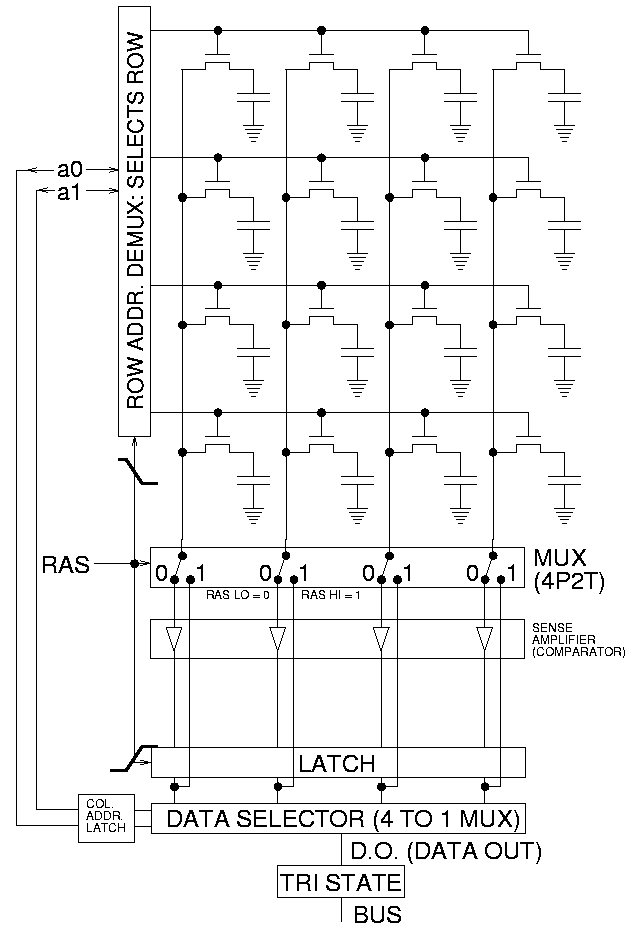
\includegraphics[width=0.4\textwidth]{Square_array_of_mosfet_cells_read.png}
\caption{ Черновик предлагаемой карты проекта}
\end{figure}

В нашем массиве цепи измерения массивны и мы не можем позволить себе ставить по одному измерителю на каждую линию, и нужно двигать наш модуль измеритель-генератор по строкам и столбцам (два модуля).\\
Предлагается использовать нечто вроде сетки из pass гейтов. Соответственно для начала предлагаю оценить насколько pass gate губителен для прохождения сигнала и измерения. Насколько сильно будет гаснуть сигнал при прохождении.
\section{Измерения}


\subsection{Конденсатор}
Предлагаю первым измерением попробовать взять просто сегнетожлектрический конденсатор и слабый резистор и попробовать попереключать его в обе стороны. Соотстветнно для этого нужно прикладывать напряжение то с одной то с другой стороны. Посмотри какой ток протекает через него при базовых значениях которые я для него вбил и при размере $500X500nM$. Напряжение переключения ты можешь задавать как параметр. Поляризация будет как и емкость зависить от площади. Можно попробовать как подключать напрямую к источнику, так и через транзистор (на рисунке).




\begin{figure}[h]
\centering
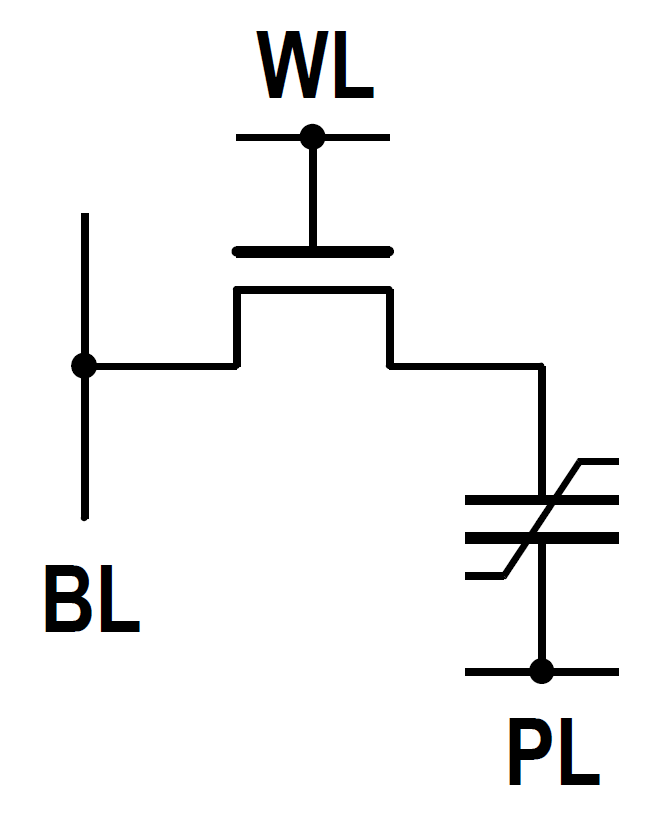
\includegraphics[width=0.3\textwidth]{FRAM-fig1.PNG}
\caption{Схема подключения конденсатора через транзистор.}
\end{figure}



\begin{figure}[h]
\centering
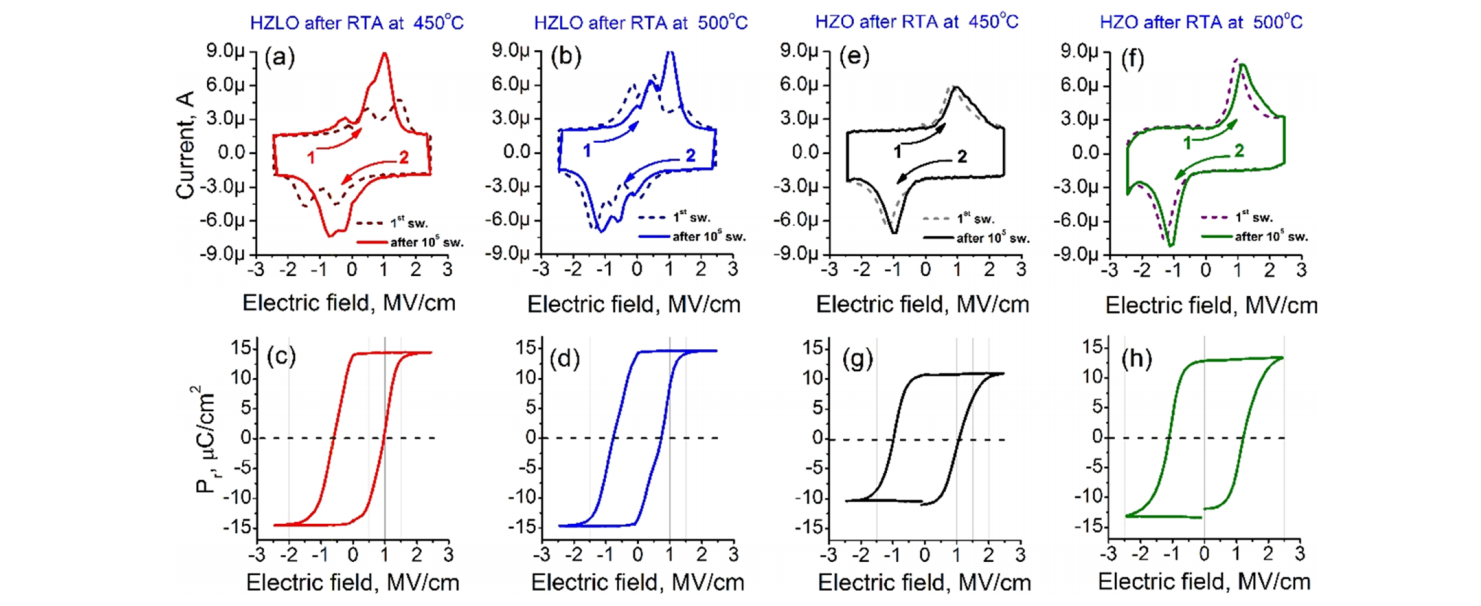
\includegraphics[width=0.5\textwidth]{segneto-graph.png}
\caption{По току переключения будут выглядить как то так.}
\end{figure}


\paragraph{Код модели}

Готовую ячейку cadence с конденсатором, ты можешь найти по адресу на сервере: \url{/home/share/mik/fram_cells/conder}.\\
Если есть проблемы с ее импортом в свой проект, используй исходный код. Он доступен в папке с этой инструкцией под названием \textbf{\textit{conder.va}}. Для создания ячейки достаточно сделать verilog A ячейку. Потом create cellview из нее.

\paragraph{Мотивация}

Постарайся особо не тратить время на этот шаг, ибо это просто тест работы модели. Данный шаг нужен чтобы понять как себя ведут сегнетоэлектрики в ответ на разные стимулы. Так же ты можешь поставить и обычный конденсатор \textit{(analoglib/cap)}. Чтобы посмотреть в чем разница. На таких размерах используй $C=10fF$ или $C=100fF$ 

\end{document}
